\documentclass[10pt]{article}
%..............................................................................
% NOTE THAT THE graphicx PACKAGE HAS TO BE CALLED BEFORE \define@key
% OR CALLED AS \RequirePackage{keyval}
%\usepackage{graphicx}

\makeatletter
\RequirePackage{keyval}
\define@key{headers}{author}{\def\Author{#1}}
\define@key{headers}{title}{\def\Title{#1}}
\define@key{headers}{major}{\def\Major{#1}}
\define@key{headers}{mentor}{\def\Mentor{#1}}
\define@key{headers}{member}{\def\Member{#1}}


\usepackage{multicol}
\columnsep 0.25in
\newcommand{\SingleCol}{\section*{}}
\newcommand{\DoubleCols}{\begin{multicols*}{2}}
\newcommand{\TripleCols}{\begin{multicols*}{3}}
\newcommand{\QuadCols}{\begin{multicols*}{4}}
\newcommand{\EndCols}{\end{multicols*}}
\newcommand{\DoubleCol}{\begin{multicols}{2}}
\newcommand{\TripleCol}{\begin{multicols}{3}}
\newcommand{\QuadCol}{\begin{multicols}{4}}
\newcommand{\EndCol}{\end{multicols}}
\doublehyphendemerits=40000
\lefthyphenmin2
\righthyphenmin2

% CONFIGURE Figure and Table ENVIRONMENT FOR multicol
\newenvironment{Figure}
  {\par\medskip\noindent\minipage{\linewidth}}
  {\endminipage\par\medskip}
\newenvironment{Table}
  {\par\medskip\noindent\minipage{\linewidth}}
  {\endminipage\par\medskip}
%

% SET FONT SIZES
\newcommand{\hfn}{\usefont{T1}{ptm}{m}{n}\fontsize{12.0}{14.0}\selectfont}
\newcommand{\hfnl}{\usefont{T1}{ptm}{m}{n}\fontsize{16.8}{22.8}\selectfont}
\newcommand{\hfs}{\usefont{T1}{ptm}{m}{n}\fontsize{9.0}{9.8}\selectfont}

% SET VERTICAL SPACE
\newcommand{\Strut}[1]{\rule{0cm}{{#1}\textwidth}}
\usepackage{wrapfig}

% FIGURE FOR END OF DOCUMENT
\newcommand{\Next}{\\[0.48em]}
\newcommand{\portrait}[5]{
\setlength{\unitlength}{1cm}
\hspace*{-1.4cm}
\begin{tabular}{ll}
\hspace*{4.0cm} &  \\
\begin{picture}(0.0,0.0)({#1},{#2})
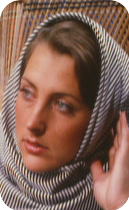
\includegraphics[scale={#3}]{./photos/portrait.png}
\end{picture} &
\parbox[t]{4.8cm}{
\hfs
\textbf{\textit{{#4}}}
{#5}
 }
\end{tabular}
}



\newcommand{\MyDocument}[1][]{%
 \setkeys{headers}{#1}
}
%..............................................................................
\usepackage[noindentafter,compact]{titlesec}
\titlespacing{\section}{0pt}{2.0ex plus 1ex minus .2ex}{0.2ex plus .2ex}
\titlespacing{\subsection}{0pt}{2.0ex plus 1ex minus .2ex}{0.2ex plus .2ex}
\titlespacing{\subsubsection}{0pt}{2.0ex plus 1ex minus .2ex}{0.2ex plus .2ex}
\titlespacing{\paragraph}{0pt}{2.0ex plus 1ex minus .2ex}{0.2ex plus .2ex}
\titlespacing{\subparagraph}{0pt}{2.0ex plus 1ex minus .2ex}{0.2ex plus .2ex}
%\renewcommand\chaptername{Chapter}
%\renewcommand\appendixname{Appendix}
\titleformat{\chapter}{\Large\bfseries}{\thechapter}{0.5em}{}
\titleformat{\section}{\normalfont\bfseries}{\thesection}{0.5em}{}
\titleformat{\subsection}{\normalfont\bfseries}{\thesubsection}{0.5em}{}
\titleformat{\subsubsection}{\normalfont\bfseries}{\thesubsubsection}{0.5em}{}
\titleformat{\paragraph}{\normalfont\bfseries}{\theparagraph}{0.5em}{}
\titleformat{\paragraph}{\normalfont\bfseries}{\thesubparagraph}{0.5em}{}
%
\renewcommand{\thesection}{\arabic{section}.}
\renewcommand{\thesubsection}{\arabic{section}.\arabic{subsection}}
\renewcommand{\thesubsubsection}{\arabic{section}.\arabic{subsection}.\arabic{subsubsection}}
%
\usepackage{amssymb,amsfonts,amsmath,amsthm,eucal}
\usepackage{graphicx}
\usepackage{caption}
\usepackage{float}
\usepackage{subcaption}
\usepackage[text={7.0in,9.5in}, top=0.75in, left=0.75in, headheight=0pt]{geometry}
\graphicspath{{figures/}} 
\usepackage{lipsum}
\usepackage{setspace}
%\onehalfspacing
\singlespacing
\usepackage{mathptmx}
%\usepackage{newtxmath}
\usepackage{makeidx}
\makeindex
\usepackage{refcount}
\usepackage{longtable}
\usepackage{multirow}
\usepackage[table,usenames,dvipsnames,x11names,svgnames]{xcolor}  % USE WITH longtable,multirow
%\usepackage{color}
\usepackage{rotate}
\usepackage{paralist}
%\usepackage{inconsolata,lmodern}
%
%\usepackage{url}
%\urlstyle{sf}
%\usepackage[linktocpage=true]{hyperref}
\definecolor{darkgreen}{rgb}{0.0,0.5,0.05}
\definecolor{darkblue}{rgb}{0.0,0.1,0.3}
\definecolor{darkred}{rgb}{0.5,0.0,0.1}
%\hypersetup{colorlinks=true,linkcolor={black},urlcolor={darkblue},citecolor={red}}
%\newcommand{\linkcolors}[3]{
%\hypersetup{colorlinks=true,linkcolor={#1},urlcolor={#2},citecolor={#3}}
%}
%
\usepackage[protrusion=true,expansion=true]{microtype}
\usepackage[font={small}]{caption}
\captionsetup[figure]{labelfont=bf}
\captionsetup[table]{labelfont=bf}
\usepackage[absolute]{textpos}
\setlength{\TPHorizModule}{1mm}
\setlength{\TPVertModule}{1mm}
%\usepackage[titletoc]{appendix}
% add dots to chapters:
%\usepackage[titles]{tocloft}
%\renewcommand{\cftchapdotsep}{\cftdotsep}
%
\usepackage{fancyhdr}
\usepackage{lastpage}
%\pagestyle{fancy}
\renewcommand{\headrulewidth}{0.0pt} % FOR TOP LINE BELOW HEADER
\renewcommand{\footrulewidth}{0.0pt} % FOR BOTTOM LINE ABOVE FOOTER
\fancyhead[R]{}
\fancyhead[L]{}
\fancyfoot[R]{}
\fancyfoot[L]{}
\fancyfoot[c]{\thepage}
%\cfoot{}                             % SET TO CLEAR PAGE NUMBERING
\usepackage{pdfpages}
\usepackage{fancybox}
\usepackage{wallpaper}
%\usepackage{background}
\usepackage{ifthen}
\usepackage{framed}

\newcommand{\pagelabel}[1]{\phantomsection\label{#1}}

%...............................................................................
% Define Urls
%\makeatletter
%\def\UrlBreaks{\do\.\do\\\do\/\do\!\do\_\do\|\do\;\do\>\do\]%no @
% \do\)\do\,\do\?\do\'\do+\do\=\do\#}%
%\def\UrlBigBreaks{\do\/\do@url@hyp}%add /
%\def\UrlSpecials{\do\/{\Url@slash}\do\ {\Url@space}\do\%{\Url@percent}\do\^^M{\Url@space}%
%   \Url@force@Tilde}%
%\def\Url@slash{\@ifnextchar/{\kern-.11em\mathchar47\kern-.15em}%
%   {\kern-.05em\mathchar47\kern-.08em\penalty\UrlBigBreakPenalty}}
%
%\makeatother
%JK\newcommand{\Urls}[1]{
%JK%\url{#1}}
%JK\href{#1}{\color{darkblue} \hspace{-0.5em} \url{#1}}}
% NO HYPERLINKS
\newcommand{\Urls}[1]{{\tt{#1}}}

%...............................................................................
\newcommand{\PutOval}[5]{ \fancyput(#1in,#2in){ \setlength{\unitlength}{#5in}\fancyoval({#3},{#4}) }}
\newcommand{\EndOval}{ \fancyput(1in,2in){ \setlength{\unitlength}{0in}\fancyoval(1,1) }}

%...............................................................................
\newcommand{\AddDraft}{
\CenterWallPaper{1}{figures/draft.pdf}
}


%...............................................................................
%\newcommand{\Rev}{
%\SetBgContents{\color{darkred} Rev: \Revision}
%\SetBgScale{1}
%\SetBgAngle{0}
%\SetBgOpacity{1}
%\SetBgPosition{current page.south west}
%\SetBgHshift{6.9in}
%\SetBgVshift{0.64in}
%}
\newcommand{\Rev}{
\fancypagestyle{plain}
{%
   \fancyhf{}%
   \fancyfoot[R]{\ifthenelse{\value{page}=1}{\bfseries \Rev}{\Rev}}
   \fancyfoot[C]{\thepage}
   \fancyfoot[R]{\textcolor{darkred}\Revision}
}
   \fancyfoot[R]{\textcolor{darkred}\Revision}
}

%\renewcommand\appendixtocname{Appendix}
\renewcommand{\tt}{\usefont{T1}{cmtt}{m}{n}\fontsize{10.0}{12.0}\selectfont}
%\def\ttdefault{blg}


%...............................................................................
%
\newcommand{\acknowledgments}[1]{
\section*{Acknowledgments}
{#1}
}
%
%
%...............................................................................
% SurfTitle
\newcommand{\mksurftitle}{
\thispagestyle{empty}
\vspace*{-0.3in}
\begin{center}
{\hfnl \Title} \\[0.1cm]
{\hfn \Author} \\[0.1cm]
{\hfn \Major} \\[0.1cm]
{\hfn \Mentor} \\[0.1cm]
\end{center}
}

%...............................................................................
% SurfAbstract
\newcommand{\mkabstract}[1]{
\noindent
\textbf{Abstract}\\
{#1}
}




%\endinput
%%
%% End of file `unh.cls'.





%...............................................................................
% Define user math commands (modify the file preamble-math.tex to suit needs):
\usepackage{relsize}
\usepackage{bigints}


\newcommand{\Reals}{\mathbb{R}}
\newcommand{\reals}{\mathbb{R}}
\newcommand{\Real}{\mathbb{R}}
\newcommand{\real}{\mathbb{R}}
\newcommand{\Field}{\mathbb{F}}
\newcommand{\field}{\mathbb{F}}
\newcommand{\Naturals}{\mathbb{N}}
\newcommand{\naturals}{\mathbb{N}}
\newcommand{\Rational}{\mathbb{Q}}
\newcommand{\rational}{\mathbb{Q}}
\newcommand{\Rationals}{\mathbb{Q}}
\newcommand{\rationals}{\mathbb{Q}}
\newcommand{\Integer}{\mathbb{Z}}
\newcommand{\integer}{\mathbb{Z}}
\newcommand{\Integers}{\mathbb{Z}}
\newcommand{\integers}{\mathbb{Z}}
\newcommand{\Complex}{\mathbb{C}}
\newcommand{\complex}{\mathbb{C}}

% Allows typing of math even in non-math mode.
\newcommand{\vfrac}[2]{\ensuremath{\frac{#1}{#2}}}


\begin{document}
\pagestyle{empty}
%...............................................................................
% The following defines the heading of the document.
% Users should modify this carefully, i.e., a missing comma or brace will cause 
% difficulties:

\MyDocument[
author          = {Jane Q.\ Student},
title           = {Poisson Kernel Estimates of Lexigraphic Matrices},
major           = {BS Applied Mathematics},
mentor          = { Faculty Mentor: Dr.\ Joseph Kolibal}
]

%These values are used throughout the document.

%...............................................................................
% User configuration options:

% Mark document as Draft (uncomment the following line) 
%\AddDraft

%...............................................................................
% The titlepage:
\mksurftitle

%...............................................................................
% The abstract:
\mkabstract{
In this study we examine the suitability of efficiently inverting, or obtaining
the solution of problems associated with a class of centrosymmetric matrices
which arise from problems associated with stochastic interpolation
on regularly spaced grids. These matrices associated with these linear
systems are full, and thus the usual range of sparse matrix solvers are
not available. In particular, the study focuses directly on the properties
of centrosymmetric matrices as a means to improve the solvability of these
linear systems, showing that for these centrosymmetric matrices of even order
it is possible to achieve a factor of 7/8 improvement in the cost of
matrix inversion using Schur complements. In addition the multiplication
of these matrices can be speeded up by a factor of two by fully utilizing
the block antisymmetry of these matrices.
}

% Start double column:
\DoubleCol
%...............................................................................
% The text of the article:
\section{Background}

A square matrix
has the same number of rows as it does
columns, and it represents a linear system in which the number
of unknowns exactly matches the number of equation, and thus it represents
a linear system which may have a unique solution.
The size of an $n\times n$  matrix is referred
to as the order of the matrix $n$, and
this equals the number of rows
or columns
in a square matrix.

Finally, in terms of notation, it will be convenient to refer to the
matrix $A$ in terms of its coefficients, using the notation $A = (a_{ij})$.
For example, if we multiply the matrix $A$ by the constant $c$, then
$c A = c (a_{ij}) = (c a_{ij})$ and we demonstrate through this notational
device that matrix  multiplication
is equivalent to multiplying each entry in the matrix by the constant $c$.
This standard notational tool will prove useful in regard to demonstrating some
properties of matrices that are needed in this study.

\section{A special matrix of interest: a centrosymmetric matrix}

A matrix with a particular structure, or a specific form  associated
with the pattern of the coefficients is called a
\textit{special matrix}.
A special matrix
need not be complicated, as in
the case of the  diagonal matrix already discussed,  or it can be much more
intricate in the layout of its coefficients in some regular pattern.
The primary focus of this study is on centrosymmetric  matrices,
although even at this level of specialization,
not every centrosymmetric matrix will be of interest to us.
The centrosymmetric matrices that are of interest are those
which arise from problems associated with stochastic interpolation.

Centrosymmetric matrices\footnote{These are sometimes referred to as perplectic matrices.}
follow a pattern in which the coefficients of the matrix are reflected about
the center of the matrix~\cite{brookes}, i.e.,
the coefficients of the matrix $A$ are rotationally symmetric
about the center. Alternatively, we can define a centrosymmetric
matrix such that  $A = EAE$,
where $E = (\textbf{\em e}_n, \textbf{\em e}_{n-1}, \ldots, \textbf{\em e}_1)$ is the exchange matrix, and $\textbf{\em e}_k$ is the $k$-th standard basis vector in $\real^n$.
In this description, the coefficients of the matrix
progress lexicographically for the
first half of the rows in the matrix,
and then regress through these same coefficients listed in
reverse lexicographic order from the bottom row to the middle row,
if the matrix is of even order. If it is of odd order, the middle row
is symmetric about its center.
Perhaps the easiest way to conceptualize this pattern is through language
using palindromes.
When read backwards, a palindrome produces the same sentence when read both
forwards and backwards as in the sentence, ``Go hang a salami, I'm a lasagna hog."


\lipsum[1-2]
\section{Developments}
\lipsum[1-1]
\smallskip

\renewcommand{\baselinestretch}{1.4}
\setlength{\tabcolsep}{5pt}
\begin{Table}
\centering
\begin{tabular}[scale=0.55]{ | l | c | c | c | c |c |}
\hline
\hline
$i$ & 1 & 2 & 3 & 4 & 5 \\
\hline
$P_i$ & 0.34 & 0.11 & 0.11 & 0.11 & 0.11 1\\
\hline
$l(P)$ & 1 & 2 & 2 & 2 & 2 \\
\hline
code$(P)$ & 0 & 10 & 11 & 12 & 20  \\
\hline
Ideal Length & 0.982    & 2.009    & 2.009 & 2.009 & 2.009  \\
\hline
\end{tabular}
\captionof{table}[Tabulated results base 3]{Tabulated results in base 3 with actual and ideal code length.}
\end{Table}
\renewcommand{\baselinestretch}{1.0}
\index{example!tables}


\lipsum[1-2]

\section{Introduction to technical writing}
This is the introduction section. This should involve a brief discussion
of the purpose of the report, what concepts are essential, and what
will be investigated. Use this template for writing your analysis
files. If you examine this file closely, it has some very useful
features in it that will set up your paper so that it has a more 
professional appearance.
You should also review the rules for typesetting \LaTeX.\ 
Be mindful of some simple rules in using English:
\begin{enumerate}
\item
Do not use the first person singular in a formal report. Use the first
person plural or the third person in a passive construction. Thus

\textit{I did this work}, is unacceptable, while,
\textit{We did this work}, or
\textit{This work was done}, are acceptable.

\item
When typesetting mathematics, use punctuation. All math equations must
read as if they were English sentences. You must end these with a period,
and put commas where needed.

\item
Keep the verb tense constant. Do not switch from past to present, and then
back again, and then back again to the present. There may be a need to
do this, however be careful when you are doing it.

\item
Avoid colloquial English.
These are formal reports. These are not email
messages to your friends. Be aware that some words in English such
as \textit{big} are colloquial, and do not appear in formal writing.
Do not use \textit{very} to modify every adjective. It is usually
meaningless.

Get a manual on English usage and style from the library, or purchase one
from the bookstore. Realize that if you plan to stay in academia, or get an
administrative position in a company or a laboratory, you have to be able
to communicate effectively. Work on this skill.
\end{enumerate}

\noindent
Then be mindful of some simple rules for typesetting \LaTeX:
\begin{enumerate}
\item
Note that the previous sentence beginning this list
is not indented since it does
not begin a new paragraph. To avoid indentation,
use the \verb+\noindent+
command.

\item
Note the \verb+\usepackage+  command which changes the font and invokes
the AMS mathematics
commands (which simplify typesetting).
Note the use of the \\
\verb+ \thispagestyle{empty}+ \\
command to avoid the printing of 
page number on the title page.

\item
Use \LaTeX commands carefully. Please review how to use math mode.
Many of the reports had math in the text that was not in math
mode. All symbols, variable, and so on are to be written in math mode.
We do not use computer science variables to write equations, either,
thus
%
%
%
\begin{equation*}
\sum_{i=1}^{upperbound} x_i^2
\end{equation*}
%
%
%
is not acceptable, while in contrast,
%
%
%
\begin{equation*}
\sum_{i=1}^{n} x_i^2
\end{equation*}
%
%
%
is acceptable. 

\item
There is no need for asterices in multiplication. Thus $ab$ or $xy$,
not $a*b$ or $x*y$.


\item
Please note that \LaTeX uses the forward and backward quotes. Thus we write
\textit{``This is a quote''}, and not \textit{"This is a quote"}.
Examine this example closely. The forward quote is written using
the \verb+`+ and not the \verb+'+ quote. The forward quote is typically
on the upper left of your keyboard, on the tilde key, and below the
Esc key.
\end{enumerate}

\subsection{Background on technical writing}

Introduce the mathematical ideas and how they are implemented in this
section. You should not have any results here.
Only introduce the mathematics that is necessary to discuss your
results. For example, the method used to compute each norm may be
important, however you may choose to either typeset the equations
or refer to these in your text, or any other reference.
You may refer to equations using a
bibliography reference generated using a bib file.



\subsection{What's in the results}

Discuss the results. This means that you provide details concerning
the numerical experiments that were performed. This section should
include graphs, tables and other supporting documentation. It should
read well, and all items discussed in the text should refer to tables,
graphs and equations using the reference command in \LaTeX and using
the format
\verb+Table~\ref{table:mytable}+,
\verb+Figure~\ref{figure:myfigure}+ to refer to tables and figures.
Equations should be referred to using the number
of the equation in parentheses, i.e., 
\verb+(\ref{eq:myequation})+.
You never use the word `equation', except at the beginning of a sentence,
in which case you use the construction:
\verb+Eq.~(\ref{eq:myequation})+.
Note that you need the 
\verb+~+, i.e., the tilde, to avoid having \LaTeX break the object across a
line. Always tie counters to their attributes using a tilde or a thin space,
e.g.,
\vspace*{0.4em}

 tied using a tilde:  \verb+in Sec.~\ref{sec:topics}+
 $\implies$ in Sec.~3.7

 tied using a thin space:  \verb+in Sec.\,\ref{sec:topics}+
 $\implies$ in Sec.\,3.7

 untied (wrong):  \verb+in Sec. \ref{sec:topics}+
 $\implies$ in Sec. 3.7

\vspace*{0.4em}
\noindent
which ties the object Sec.\ to the counter. Not only is the space too large
after the period when there is no tie, but there is the danger that the
word, Sec., will go at the end of one line, and the number 3.7 at the start
of a new line.


When doing numerical studies, you must present the results of all of your
numerical investigations. For the case of polynomial interpolation,
at the very least these results should have examined the behaviour of
the polynomials interpolated on $2^k$ points, where $k = 2, 3, \ldots, n$,
where $n$ is sufficiently large so as to be able to determine numerically
whether convergence was achieved. A value of $n = 5$, or $n=10$ is
usually insufficient.

Focus on the error. Numerical methods are approximations. They introduce
error. Examine the errors, and attempt to understand where they are
coming from. Examine issues of computational efficiency, and other
topics as appropriate. Time your results when you run the codes.
You can always choose not to use the timing results, however if they
show something important, then you can use it.



\subsection{What's in the conclusion}

Be brief, however one sentence is not sufficient. Try to concisely
summarize what was discussed in the results. Avoid rewriting the
results section. Someone reading your report should be able to 
understand the writeup from what is written in this section.
This is one of the most important parts of your report (and probably
the only one your supervisor or manager will ever read, so you might
as well learn to write it effectively).






\section{Using figures}
We demonstrate a technique to set up and configure
a figure using the {\tt \verb+\includegraphics+} command embedded into
the picture environment embedded into the figure environment.
The picture environment is needed to control the spacing, while the
figure environment is needed to control the floating of the figures
in the document. Note that you can refer to the figure with its
label, i.e., in Figure~\ref{fig:sample} you have the setup of the figure.
Note that you need to create the figures so that the labels and legends
scale well with the fonts being used after you have scaled the figure.
The examples in Fig.\,\ref{fig:sheet} and Fig.\,\ref{fig:sample} should
be examined in detail as the axes labels are not generated with the
figures. Instead, they are added as overlays using the
{\tt \verb+\put+} command in the {\tt picture} environment.

 
%..............................................................................
% SETUP FIGURE USING STANDARD FIGURE ENVIRONMENT.
% NOTE THAT [H] IS THE ONLY ALLOWABLE OPTION.
\setlength{\unitlength}{1cm} 
\begin{figure}[H]
\begin{picture}(0.0,6.0)(-1.2,-0.1) 
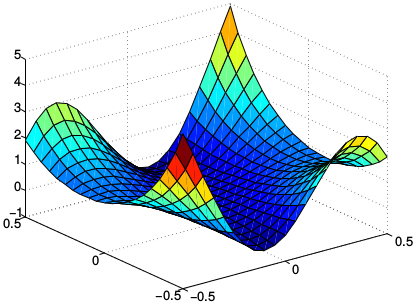
\includegraphics[scale=0.50]{./figures/sheet}
%\put(-10.8,4.2){\makebox(0,0){$f(x,y)$ }} 
\put(-7.9,2.8){\makebox(0,0){$f(x,y)$ }} 
\put(-6.5,0.5){\makebox(0,0){$x$ }} 
\put(-1.6,0.2){\makebox(0,0){$y$ }} 
\end{picture} 
\captionof{figure}{Example of using a raster image
which is scaled and annotated with axes.
\label{fig:sheet} 
} 
\end{figure}
\lipsum[8-9]

\subsection{More nonsense text}
\lipsum[15-16]


% SETUP FIGURE USING ./unhpreamble.tex FIGURE ENVIRONMENT.
% NOTE THAT THERE IS NO PLACEMENT VALUE.

% BREAK OUT OF TWO COLUMN MODE INTO SINGLE COLUMN MODE.
\EndCol
\SingleCol
%
% DEFINE FONT FOR FIGURE.
\newcommand{\Hfs}{\usefont{T1}{phv}{m}{n}\fontsize{8.4}{8.0}\selectfont}
%
\setlength{\unitlength}{1cm}
\begin{Figure}
\begin{picture}(0.0,7.7)(-1.5,0.0)
\put(0.2,3.0){\rotatebox[origin=lb]{90}{
 {\Hfs Estimate of} \ ${\cal I}(N)$ }}
\put(14.1,3.0){\rotatebox[origin=lb]{90}{
  {\Hfs Error}, $\varepsilon = \left| {\cal V} - {\cal I}(N) \right|$}}
\put(7.0,0.0){\makebox(0,0){$N$ }}
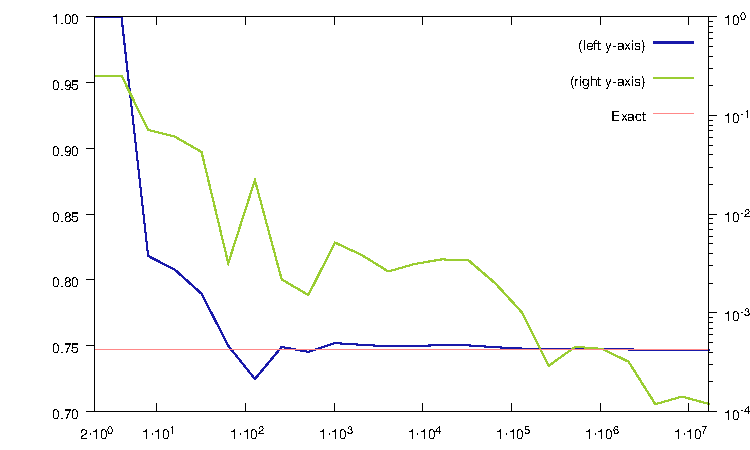
\includegraphics[scale=1.1]{./figures/logfigs/integral}
\end{picture}
\captionof{figure}{
An approximation ${\cal I}(N)$ to the value of the integral
for $\int_0^1 e^{x^2}dx$ obtained using a Monte Carlo approach.
The estimate for ${\cal I}(N)$ is a function of the number
of samples $N$, and the value of $I \approx 0.7468241328 \equiv {\cal V}$
was obtained using Wolfram Alpha$^\circledR$.
\label{fig:sample}
}
\end{Figure}
%
% GO BACK TO TWO COLUMN MODE.
\DoubleCol






\subsection{Using another figure}
\lipsum[3-4]

\subsection{Even more results}
\lipsum[9-10]
\section{Conclusions}
Everything we have done is completely correct based on the theory
of everything.
\index{theory of everything}
\lipsum[11-12]
Where can we find information about this thesis style? 
Go to \Urls{http://math.newhaven.edu/mathphysics}.


%...............................................................................
% Bibliography references that are not specifically cited:
%...............................................................................
%
%
% YOU NEED TO CITE THOSE ARTICLES THAT ARE IN THE BIB FILE IF THEY
% ARE TO BE INCLUDED:
\nocite{Bozick}
\nocite{DowdCoury}
\nocite{Dynarski}
\nocite{Johnsonetal}
\nocite{Kim}
\nocite{MantheiGilmore}
\nocite{McPhersonSchapiro}


% The Bibliography
\bibliographystyle{plain}
\bibliography{SURFc}


\acknowledgments{
I would like to thank my advisor Dr.\ Strange Strangelove for
guidance throughout the project, and Dr.\ Tom Clown for the help with
everything else, and everyone else for financial support.
}




% NOTE THAT THE FIGURE MUST BE in ./photos/portrait.png, AND SHOULD HAVE AN
% x/y ASPECT RATIO OF ABOUT 0.6. THE EXAMPLE IS 129x210 pixels, AND SO IS
% SCALED BY A FACTOR OF 0.6.
%
% USE Imagemagick TO CREATED ROUNDED CORNERS (DONE BY SCRIPT IN ./bin/mkborder).
%
\portrait
{-1.4}   % xoffset for image in cm
{4.2}    % yoffset for image in cm
{0.6}    % scale factor applied to image
%
% DESCRIPTON ON RIGHT. IT SHOULD BE SHORT.
%
{\Author}
{is a senior in the Department of Mathematics and Physics studying Applied Mathematics at UNH
\Next
Her interests are in the development of algorithms for pontificating on
mathematics, and is interested in an academic career in mathematics.
\Next
She has published one student article and has given two student
presentations during the May, 2014 MAA Conference at UNCC, Topeka, AZ.
}


% ADD VERTICAL SPACE. ADJUST VALUE INSIDE BRACES, OR COMMENT OUT TO GET
% A FLUSH BOTTOM LAST PAGE.
%\Strut{0.6}


% End double column.
\EndCol



\end{document}
